\documentclass[aspectratio=169,10pt]{beamer}

\usepackage{iftex}
\providecommand{\dunenoirsetupfonts}{}
\newcommand{\DuneNoirLocalFontPath}{fonts}

\newcommand{\DuneNoirMonoFallback}{%
  \IfFontExistsTF{JetBrainsMono Nerd Font Propo}{
    \setmonofont{JetBrainsMono Nerd Font Propo}[Scale=0.92]
  }{
    \IfFontExistsTF{JetBrainsMono Nerd Font}{
      \setmonofont{JetBrainsMono Nerd Font}[Scale=0.92]
    }{
      \setmonofont{Courier New}[Scale=0.92]
    }
  }
}

\newcommand{\DuneNoirSansFallback}{%
  \IfFontExistsTF{IBM Plex Sans}{
    \setsansfont{IBM Plex Sans}
    \setmainfont{IBM Plex Sans}
  }{
    \IfFontExistsTF{Helvetica Neue}{
      \setsansfont{Helvetica Neue}
      \setmainfont{Helvetica Neue}
    }{
      \setsansfont{Arial}
      \setmainfont{Arial}
    }
  }
}

\newcommand{\DuneNoirUseHelvetica}{%
  \renewcommand{\dunenoirsetupfonts}{%
    \IfFontExistsTF{Helvetica Neue}{
      \setsansfont{Helvetica Neue}
      \setmainfont{Helvetica Neue}
    }{
      \IfFontExistsTF{Helvetica}{
        \setsansfont{Helvetica}
        \setmainfont{Helvetica}
      }{
        \DuneNoirSansFallback
      }
    }
    \DuneNoirMonoFallback
  }%
}

\newcommand{\DuneNoirUseOpenSans}{%
  \renewcommand{\dunenoirsetupfonts}{%
    \IfFileExists{\DuneNoirLocalFontPath/OpenSans.ttf}{
      \setsansfont{Open Sans Custom}[
        Path=\DuneNoirLocalFontPath/,
        UprightFont={OpenSans.ttf},
        ItalicFont={OpenSans-Italic.ttf},
        BoldFont={OpenSans.ttf},
        BoldItalicFont={OpenSans-Italic.ttf},
        BoldFeatures={FakeBold=1.45},
        BoldItalicFeatures={FakeBold=1.45}
      ]
      \setmainfont{Open Sans Custom}[
        Path=\DuneNoirLocalFontPath/,
        UprightFont={OpenSans.ttf},
        ItalicFont={OpenSans-Italic.ttf},
        BoldFont={OpenSans.ttf},
        BoldItalicFont={OpenSans-Italic.ttf},
        BoldFeatures={FakeBold=1.45},
        BoldItalicFeatures={FakeBold=1.45}
      ]
    }{
      \DuneNoirSansFallback
    }
    \DuneNoirMonoFallback
  }%
}

\newcommand{\DuneNoirUseDosis}{%
  \renewcommand{\dunenoirsetupfonts}{%
    \IfFileExists{\DuneNoirLocalFontPath/Dosis.ttf}{
      \setsansfont{Dosis Custom}[
        Path=\DuneNoirLocalFontPath/,
        UprightFont={Dosis.ttf},
        ItalicFont={Dosis.ttf},
        BoldFont={Dosis.ttf},
        BoldItalicFont={Dosis.ttf},
        ItalicFeatures={FakeSlant=0.16},
        BoldFeatures={FakeBold=1.6},
        BoldItalicFeatures={FakeBold=1.6,FakeSlant=0.16}
      ]
      \setmainfont{Dosis Custom}[
        Path=\DuneNoirLocalFontPath/,
        UprightFont={Dosis.ttf},
        ItalicFont={Dosis.ttf},
        BoldFont={Dosis.ttf},
        BoldItalicFont={Dosis.ttf},
        ItalicFeatures={FakeSlant=0.16},
        BoldFeatures={FakeBold=1.6},
        BoldItalicFeatures={FakeBold=1.6,FakeSlant=0.16}
      ]
    }{
      \DuneNoirSansFallback
    }
    \DuneNoirMonoFallback
  }%
}

\newcommand{\DuneNoirUseKoHo}{%
  \renewcommand{\dunenoirsetupfonts}{%
    \IfFileExists{\DuneNoirLocalFontPath/KoHo-Regular.ttf}{
      \setsansfont{KoHo Custom}[
        Path=\DuneNoirLocalFontPath/,
        UprightFont={KoHo-Regular.ttf},
        BoldFont={KoHo-Bold.ttf},
        ItalicFont={KoHo-Italic.ttf},
        BoldItalicFont={KoHo-BoldItalic.ttf}
      ]
      \setmainfont{KoHo Custom}[
        Path=\DuneNoirLocalFontPath/,
        UprightFont={KoHo-Regular.ttf},
        BoldFont={KoHo-Bold.ttf},
        ItalicFont={KoHo-Italic.ttf},
        BoldItalicFont={KoHo-BoldItalic.ttf}
      ]
    }{
      \DuneNoirSansFallback
    }
    \DuneNoirMonoFallback
  }%
}

\DuneNoirUseHelvetica
\makeatletter
\mode<presentation>
\RequirePackage{iftex}
\RequirePackage{tikz}
\usetikzlibrary{calc,positioning}
\usecolortheme{default}
\useinnertheme{default}
\useoutertheme{default}

% --------------------------------------
% TYPOGRAPHY
% --------------------------------------
\setbeamerfont{normal text}{size=\small}
\setbeamerfont{title}{size=\Huge,series=\bfseries}
\setbeamerfont{subtitle}{size=\large}
\setbeamerfont{author}{size=\normalsize,series=\bfseries}
\setbeamerfont{date}{size=\small}
\setbeamerfont{frametitle}{size=\LARGE,series=\bfseries}
\setbeamerfont{block title}{size=\normalsize,series=\bfseries}
\setbeamerfont{block body}{size=\small}
\setbeamerfont{headline}{size=\scriptsize,series=\bfseries}
\setbeamerfont{footline}{size=\scriptsize}

% --------------------------------------
% COLORS
% --------------------------------------
\definecolor{noirbg}{HTML}{131B24}
\definecolor{noirpanel}{HTML}{1C2834}
\definecolor{noirpanelalt}{HTML}{2A3948}
\definecolor{noirtitlebar}{HTML}{22303D}
\definecolor{noirline}{HTML}{556779}
\definecolor{noirtext}{HTML}{ECF1F4}
\definecolor{noirmuted}{HTML}{C4CDD5}
\definecolor{duneorange}{HTML}{F2682B}
\definecolor{noircyan}{HTML}{92DDF2}
\definecolor{noirmint}{HTML}{EAE0CC}

\setbeamercolor{normal text}{fg=noirtext,bg=noirbg}
\setbeamercolor{title}{fg=white}
\setbeamercolor{subtitle}{fg=noirmuted}
\setbeamercolor{author}{fg=noircyan}
\setbeamercolor{date}{fg=noirmuted}
\setbeamercolor{frametitle}{fg=white,bg=noirbg}
\setbeamercolor{headline}{fg=noirmuted,bg=noirbg}
\setbeamercolor{footline}{fg=noirmuted,bg=noirbg}
\setbeamercolor{section in toc}{fg=noirtext,bg=noirbg}
\setbeamercolor{caption name}{fg=noirmuted}
\setbeamercolor{itemize item}{fg=duneorange}
\setbeamercolor{itemize subitem}{fg=noircyan}
\setbeamercolor{enumerate item}{fg=duneorange}

\setbeamercolor{block title}{fg=noircyan,bg=noirtitlebar}
\setbeamercolor{block body}{fg=noirtext,bg=noirpanel}
\setbeamercolor{block title alerted}{fg=duneorange!85!white,bg=noirtitlebar}
\setbeamercolor{block body alerted}{fg=noirtext,bg=noirpanelalt}
\setbeamercolor{block title example}{fg=noirmint,bg=noirtitlebar}
\setbeamercolor{block body example}{fg=noirtext,bg=noirpanelalt}
\setbeamercolor{panel}{fg=noirtext,bg=noirpanel}
\setbeamercolor{panel alt}{fg=noirtext,bg=noirpanelalt}
\setbeamercolor{panel accent}{fg=noirbg,bg=noircyan}
\setbeamercolor{panel soft}{fg=noirbg,bg=noirpanelalt!18!white}

\setbeamertemplate{blocks}[rounded][shadow=false]
\setbeamersize{text margin left=0.8cm, text margin right=0.8cm}
\setlength{\leftmargini}{1.2em}
\setlength{\leftmarginii}{1.1em}
\setlength{\parskip}{0.22em}

% --------------------------------------
% FONT SETUP
% --------------------------------------
\usefonttheme{professionalfonts}
\ifPDFTeX
  \usepackage[scaled]{helvet}
  \renewcommand*\familydefault{\sfdefault}
  \usepackage[T1]{fontenc}
\else
  \usepackage{fontspec}
  \defaultfontfeatures{Ligatures=TeX,Scale=MatchLowercase}
  \providecommand{\dunenoirsetupfonts}{%
    \IfFontExistsTF{IBM Plex Sans}{
      \setsansfont{IBM Plex Sans}
      \setmainfont{IBM Plex Sans}
    }{
      \IfFontExistsTF{Helvetica Neue}{
        \setsansfont{Helvetica Neue}
        \setmainfont{Helvetica Neue}
      }{
        \setsansfont{Arial}
        \setmainfont{Arial}
      }
    }
    \IfFontExistsTF{JetBrainsMono Nerd Font Propo}{
      \setmonofont{JetBrainsMono Nerd Font Propo}[Scale=0.92]
    }{
      \IfFontExistsTF{JetBrainsMono Nerd Font}{
        \setmonofont{JetBrainsMono Nerd Font}[Scale=0.92]
      }{
        \setmonofont{Courier New}[Scale=0.92]
      }
    }
  }
  \dunenoirsetupfonts
  \renewcommand*\familydefault{\sfdefault}
\fi

% --------------------------------------
% LISTS AND TITLES
% --------------------------------------
\setbeamertemplate{navigation symbols}{}
\setbeamertemplate{itemize item}{\color{duneorange}\raisebox{0.18ex}{\scriptsize$\blacktriangleright$}}
\setbeamertemplate{itemize subitem}{\color{noircyan}\raisebox{0.18ex}{\tiny$\blacktriangleright$}}
\setbeamertemplate{frametitle}{%
  \vspace*{0.8mm}%
  {\usebeamerfont{frametitle}\usebeamercolor[fg]{frametitle}\insertframetitle\par}%
  \vspace{0.4mm}%
}

% --------------------------------------
% BACKGROUND
% --------------------------------------
\addtobeamertemplate{background canvas}{%
  \begin{tikzpicture}[remember picture,overlay]
    \fill[noirbg] (current page.south west) rectangle (current page.north east);
    \fill[noirpanelalt] ($(current page.north east)+(-4.8,0)$) rectangle ($(current page.north east)+(0,-1.05)$);
    \draw[noirline, line width=0.7pt] ($(current page.south west)+(0.8,0.78)$) -- ($(current page.south east)+(-0.8,0.78)$);
    \fill[noircyan!14] ($(current page.south east)+(-3.4,0.86)$) rectangle ++(1.55,0.07);
  \end{tikzpicture}
}{}

% --------------------------------------
% HEADLINE AND FOOTLINE
% --------------------------------------
\setbeamertemplate{headline}{%
  \leavevmode%
  \begin{beamercolorbox}[wd=\paperwidth,ht=8.2mm,dp=0mm,leftskip=0.8cm,rightskip=0.8cm]{headline}%
    \vspace{1.1mm}%
    {\usebeamerfont{headline}\textcolor{noirmuted}{\insertshorttitle}}%
  \end{beamercolorbox}%
}

\setbeamertemplate{footline}{%
  \leavevmode%
  \begin{beamercolorbox}[wd=\paperwidth,ht=7.6mm,dp=2.2mm,leftskip=0.8cm,rightskip=0.8cm]{footline}%
    \footerdunelogo\hspace{0.45em}{\usebeamerfont{footline}\textcolor{noirmuted}{\talkdate}}%
    \hfill%
    {\usebeamerfont{footline}\textcolor{duneorange}{\bfseries\insertframenumber}\textcolor{noirmuted}{/\inserttotalframenumber}}%
  \end{beamercolorbox}%
}

% --------------------------------------
% DATE HANDLING
% --------------------------------------
\newcommand{\talkdate}{%
  \@ifundefined{mydate}
  {\today}
  {\mydate}
}
\newcommand{\footerdunelogo}{%
  \IfFileExists{logos/logosolo.png}{%
    \tikz[baseline=-0.55ex]\node[opacity=0.42,inner sep=0pt]{%
      
\includegraphics[height=0.26cm]{logos/logosolo.png}%
    };%
  }{}%
}

% --------------------------------------
% TITLE PAGE
% --------------------------------------
\setbeamertemplate{title page}{%
  \begin{tikzpicture}[remember picture,overlay]
    \fill[noirbg] (current page.south west) rectangle (current page.north east);
    \fill[noirpanelalt] (current page.north west) rectangle ($(current page.north east)+(0,-2.65)$);
    \fill[duneorange] ($(current page.north west)+(0.8,-0.62)$) rectangle ++(1.5,0.08);
    \fill[noircyan] ($(current page.south east)+(-2.8,0.8)$) rectangle ++(1.9,0.08);
    \IfFileExists{logos/DUNElogo_white.png}{%
      \node[anchor=south east,opacity=0.13] at ($(current page.south east)+(-0.55,1.48)$) {%
        
\includegraphics[width=0.33\paperwidth]{logos/DUNElogo_white.png}%
      };
    }{}%
    \IfFileExists{logos/FNAL-Logo-NAL-Light.png}{%
      \node[anchor=south east] at ($(current page.south east)+(-0.92,0.82)$) {%
        
\includegraphics[height=0.45cm]{logos/FNAL-Logo-NAL-Light.png}%
      };
    }{%
      \IfFileExists{logos/FNAL-Logo-NAL-Blue.png}{%
        \node[anchor=south east] at ($(current page.south east)+(-0.92,0.82)$) {%
          
\includegraphics[height=0.45cm]{logos/FNAL-Logo-NAL-Blue.png}%
        };
      }{}%
    }%
  \end{tikzpicture}
  \vspace*{2.85cm}
  {\usebeamerfont{title}\usebeamercolor[fg]{title}\inserttitle\par}
  \vspace{3mm}
  {\usebeamerfont{subtitle}\usebeamercolor[fg]{subtitle}\insertsubtitle\par}
  \vspace{9mm}
  {\usebeamerfont{author}\usebeamercolor[fg]{author}\insertauthor\par}
  \vspace{1mm}
  {\usebeamerfont{date}\usebeamercolor[fg]{date}\insertdate\par}
  \vfill
}

\mode<all>

\makeatother

\ifPDFTeX
  \usepackage[T1]{fontenc}
  \usepackage[utf8]{inputenc}
\fi

\usepackage{amsmath,amssymb}
\usepackage{array,booktabs,tabularx}
\usepackage{graphicx}
\usepackage{hyperref}
\usepackage{tikz}
\usetikzlibrary{arrows.meta,calc,positioning,fit,shapes.geometric}

\graphicspath{{figures/pptx/}{../daphne_firmware_architecture_assets/output/}{../daphne_deadtime_apr2026/figures/}}

\title[DAPHNE Electronics Integration]{DAPHNE Electronics Integration}
\subtitle{Status update: cold-box mezzanine evidence\\DAQ handoff, and PRR gates}
\author[Manuel Arroyave]{\texorpdfstring{Manuel Arroyave\\{\small on behalf of the PDS and DAQ groups}}{Manuel Arroyave on behalf of the PDS and DAQ groups}}
\date{Lead, South Dakota - Wednesday, May 20, 2026}
\newcommand{\mydate}{Lead, South Dakota - May 20, 2026}

\definecolor{okgreen}{HTML}{8FD6A9}
\definecolor{warnyellow}{HTML}{E7C547}
\definecolor{riskred}{HTML}{F28B82}
\definecolor{duneorangesoft}{HTML}{F7A072}

\setbeamercolor{panel evidence}{fg=noirbg,bg=noirmint}
\setbeamercolor{panel hardware}{fg=noirbg,bg=duneorangesoft}
\setbeamercolor{panel integration}{fg=noirbg,bg=noircyan!74!white}
\setbeamercolor{panel prr}{fg=noirbg,bg=noirmint}
\setbeamercolor{panel accent}{fg=noirbg,bg=duneorangesoft}

\setbeamertemplate{title page}{%
  \begin{tikzpicture}[remember picture,overlay]
    \fill[noirbg] (current page.south west) rectangle (current page.north east);
    \fill[noirpanelalt] (current page.north west) rectangle ($(current page.north east)+(0,-2.65)$);
    \fill[duneorange] ($(current page.north west)+(0.8,-0.82)$) rectangle ++(1.5,0.08);
    \fill[noircyan] ($(current page.south east)+(-2.8,0.8)$) rectangle ++(1.9,0.08);
    \IfFileExists{logos/DUNElogo_white.png}{%
      \node[anchor=south east,opacity=0.13] at ($(current page.south east)+(-0.55,1.48)$) {%
        
\includegraphics[width=0.33\paperwidth]{logos/DUNElogo_white.png}%
      };
    }{}%
    \IfFileExists{logos/FNAL-Logo-NAL-Light.png}{%
      \node[anchor=south east] at ($(current page.south east)+(-0.92,0.82)$) {%
        
\includegraphics[height=0.45cm]{logos/FNAL-Logo-NAL-Light.png}%
      };
    }{}%
    \node[anchor=north west,text width=0.86\paperwidth] at ($(current page.north west)+(0.8,-0.96)$) {%
      {\usebeamerfont{title}\usebeamercolor[fg]{title}\inserttitle\par}%
    };
    \node[anchor=north west,text width=0.55\paperwidth] at ($(current page.north west)+(0.8,-4.12)$) {%
      {\usebeamerfont{subtitle}\usebeamercolor[fg]{subtitle}\insertsubtitle\par}%
    };
    \node[anchor=north west,text width=0.55\paperwidth] at ($(current page.north west)+(0.8,-6.45)$) {%
      {\usebeamerfont{author}\usebeamercolor[fg]{author}\insertauthor\par}
      \vspace{1mm}
      {\usebeamerfont{date}\usebeamercolor[fg]{date}\insertdate\par}%
    };
  \end{tikzpicture}%
}

\newcommand{\eyebrow}[1]{{\color{noircyan}\small\bfseries #1\par}}
\newcommand{\tinycite}[1]{{\color{noirmuted}\tiny Source: #1\par}}

\newcommand{\panelbox}[3][panel]{%
  \begin{beamercolorbox}[wd=\linewidth,sep=5pt,rounded=true]{#1}
    {\usebeamercolor[fg]{#1}\bfseries #2\par}
    \vspace{0.35mm}
    {\usebeamercolor[fg]{#1}\footnotesize #3\par}
  \end{beamercolorbox}
}

\newcommand{\statcard}[3][panel alt]{%
  \begin{beamercolorbox}[wd=\linewidth,sep=5pt,rounded=true]{#1}
    {\usebeamercolor[fg]{#1}\bfseries #2\par}
    \vspace{0.35mm}
    {\usebeamercolor[fg]{#1}\scriptsize #3\par}
  \end{beamercolorbox}
}

\newcommand{\plotbox}[2]{%
  {\centering\includegraphics[width=\linewidth,height=#1,keepaspectratio]{#2}\par}%
}

\newcommand{\figurebreath}{\vspace{2.4mm}}
\newcommand{\contentdrop}{\vspace*{3mm}}
\newcommand{\softcontentdrop}{\vspace*{2mm}}
\newcommand{\microcontentdrop}{\vspace*{1mm}}

\newcommand{\fixedpanelbox}[4][panel]{%
  \begin{beamercolorbox}[wd=\linewidth,sep=5pt,rounded=true]{#1}
    \begin{minipage}[t][#2][t]{\dimexpr\linewidth-10pt\relax}
      \raggedright
      {\usebeamercolor[fg]{#1}\bfseries #3\par}
      \vspace{0.35mm}
      {\usebeamercolor[fg]{#1}\footnotesize #4\par}
    \end{minipage}
  \end{beamercolorbox}
}

\newcommand{\fixedstatcard}[4][panel alt]{%
  \begin{beamercolorbox}[wd=\linewidth,sep=5pt,rounded=true]{#1}
    \begin{minipage}[t][#2][t]{\dimexpr\linewidth-10pt\relax}
      \raggedright
      {\usebeamercolor[fg]{#1}\bfseries #3\par}
      \vspace{0.35mm}
      {\usebeamercolor[fg]{#1}\scriptsize #4\par}
    \end{minipage}
  \end{beamercolorbox}
}

\newcommand{\fixedlargepanelbox}[4][panel]{%
  \begin{beamercolorbox}[wd=\linewidth,sep=5pt,rounded=true]{#1}
    \begin{minipage}[t][#2][t]{\dimexpr\linewidth-10pt\relax}
      \raggedright
      {\usebeamercolor[fg]{#1}\bfseries #3\par}
      \vspace{0.35mm}
      {\usebeamercolor[fg]{#1}\small #4\par}
    \end{minipage}
  \end{beamercolorbox}
}

\newcommand{\fixedxlargepanelbox}[4][panel]{%
  \begin{beamercolorbox}[wd=\linewidth,sep=4pt,rounded=true]{#1}
    \begin{minipage}[t][#2][t]{\dimexpr\linewidth-8pt\relax}
      \raggedright
      {\usebeamercolor[fg]{#1}\bfseries #3\par}
      \vspace{0.35mm}
      {\usebeamercolor[fg]{#1}\fontsize{9.4}{10.8}\selectfont #4\par}
    \end{minipage}
  \end{beamercolorbox}
}

\newcommand{\statusdot}[2]{%
  \textcolor{#1}{\rule{0.9em}{0.9em}}\hspace{0.35em}{#2}%
}

\tikzset{
  flowbox/.style={
    draw=noirline,
    fill=noirpanelalt,
    text=noirtext,
    rounded corners=4pt,
    align=center,
    text width=2.55cm,
    minimum height=0.88cm,
    inner sep=4pt,
    font=\scriptsize
  },
  flowboxwide/.style={
    flowbox,
    text width=3.15cm
  },
  flowmint/.style={flowboxwide, draw=noirmint, fill=noirmint, text=noirbg},
  flowcyan/.style={flowboxwide, draw=noircyan!90!white, fill=noircyan!74!white, text=noirbg},
  floworange/.style={flowboxwide, draw=duneorange, fill=duneorangesoft, text=noirbg},
  arrow/.style={-Latex, line width=0.8pt, draw=noircyan},
  warnarrow/.style={-Latex, line width=0.85pt, draw=duneorange},
  smallnote/.style={align=center, font=\tiny, text=noirmuted}
}

\newcommand{\systemDiagram}{%
\resizebox{0.88\linewidth}{!}{%
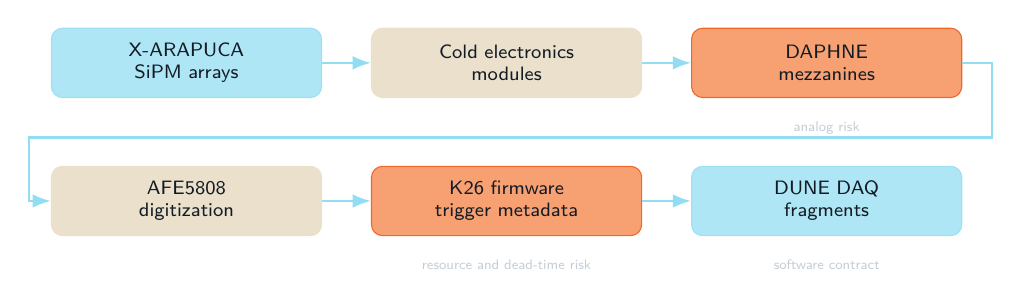
\begin{tikzpicture}[node distance=0.86cm and 0.62cm]
  \node[flowcyan] (det) {X-ARAPUCA\\SiPM arrays};
  \node[flowmint, right=of det] (cold) {Cold electronics\\modules};
  \node[floworange, right=of cold] (mezz) {DAPHNE\\mezzanines};
  \node[flowmint, below=of det] (afe) {AFE5808\\digitization};
  \node[floworange, right=of afe] (fw) {K26 firmware\\trigger metadata};
  \node[flowcyan, right=of fw] (daq) {DUNE DAQ\\fragments};
  \draw[arrow] (det) -- (cold);
  \draw[arrow] (cold) -- (mezz);
  \draw[arrow] (mezz.east) -- ++(0.38cm,0) |- ([xshift=-0.28cm,yshift=0.36cm]afe.north west) -- ([xshift=-0.28cm]afe.west) -- (afe.west);
  \draw[arrow] (afe) -- (fw);
  \draw[arrow] (fw) -- (daq);
  \node[smallnote, below=0.18cm of mezz] {analog risk};
  \node[smallnote, below=0.18cm of fw] {resource and dead-time risk};
  \node[smallnote, below=0.18cm of daq] {software contract};
\end{tikzpicture}
}%
}

\newcommand{\daqDiagram}{%
\resizebox{0.88\linewidth}{!}{%
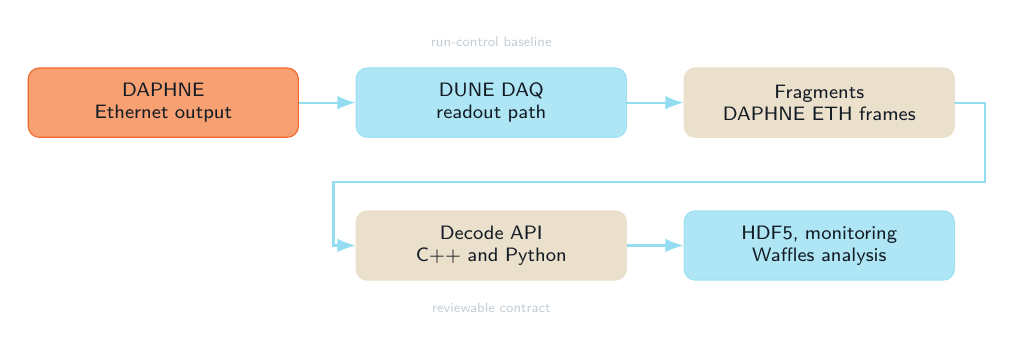
\begin{tikzpicture}[node distance=0.72cm and 0.72cm]
  \node[floworange] (hw) {DAPHNE\\Ethernet output};
  \node[flowcyan, right=of hw] (readout) {DUNE DAQ\\readout path};
  \node[flowmint, right=of readout] (frag) {Fragments\\DAPHNE ETH frames};
  \node[flowmint, below=0.92cm of readout] (decode) {Decode API\\C++ and Python};
  \node[flowcyan, right=of decode] (analysis) {HDF5, monitoring\\Waffles analysis};
  \draw[arrow] (hw) -- (readout);
  \draw[arrow] (readout) -- (frag);
  \draw[arrow] (frag.east) -- ++(0.38cm,0) |- ([xshift=-0.28cm,yshift=0.36cm]decode.north west) -- ([xshift=-0.28cm]decode.west) -- (decode.west);
  \draw[arrow] (decode) -- (analysis);
  \node[smallnote, below=0.16cm of decode] {reviewable contract};
  \node[smallnote, above=0.14cm of readout] {run-control baseline};
\end{tikzpicture}
}%
}

\newcommand{\pdsRunDiagram}{%
\resizebox{0.86\linewidth}{!}{%
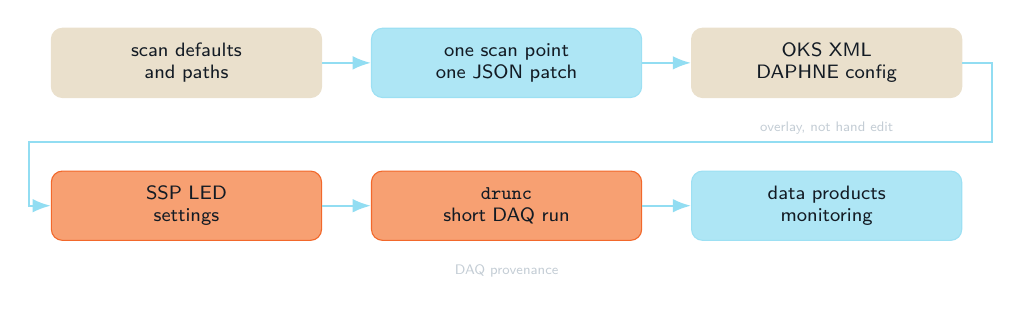
\begin{tikzpicture}[node distance=0.70cm and 0.62cm]
  \node[flowmint] (defaults) {scan defaults\\and paths};
  \node[flowcyan, right=of defaults] (point) {one scan point\\one JSON patch};
  \node[flowmint, right=of point] (oks) {OKS XML\\DAPHNE config};
  \node[floworange, below=0.92cm of defaults] (led) {SSP LED\\settings};
  \node[floworange, right=of led] (run) {\texttt{drunc}\\short DAQ run};
  \node[flowcyan, right=of run] (products) {data products\\monitoring};
  \draw[arrow] (defaults) -- (point);
  \draw[arrow] (point) -- (oks);
  \draw[arrow] (oks.east) -- ++(0.38cm,0) |- ([xshift=-0.28cm,yshift=0.36cm]led.north west) -- ([xshift=-0.28cm]led.west) -- (led.west);
  \draw[arrow] (led) -- (run);
  \draw[arrow] (run) -- (products);
  \node[smallnote, below=0.18cm of oks] {overlay, not hand edit};
  \node[smallnote, below=0.18cm of run] {DAQ provenance};
\end{tikzpicture}
}%
}

% Native TikZ replacement for
% ../daphne_firmware_architecture_assets/output/runtime_dataflow.dot.
\newcommand{\runtimeDataflowDiagram}{%
\resizebox{0.90\linewidth}{!}{%
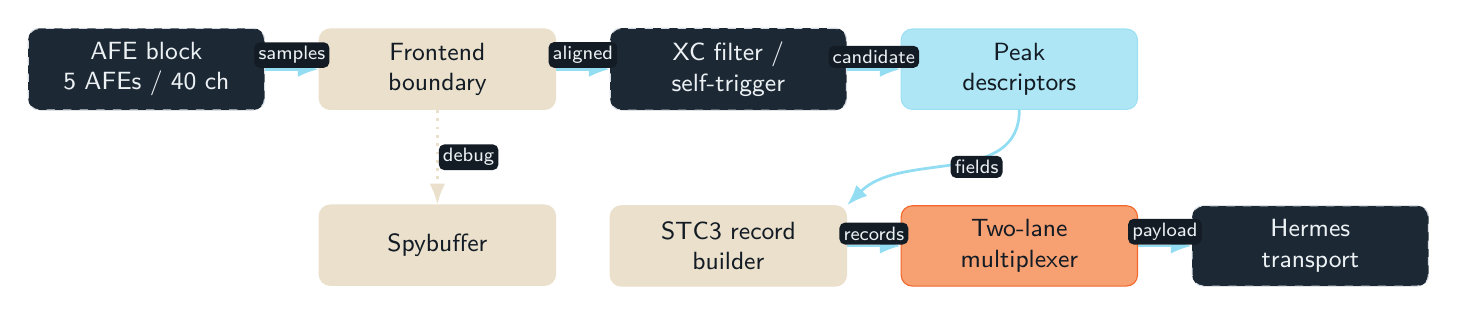
\begin{tikzpicture}[
  node distance=0.78cm and 0.68cm,
  runtime/.style={
    draw=noirline,
    fill=noirpanelalt,
    text=noirtext,
    rounded corners=4pt,
    align=center,
    text width=2.65cm,
    minimum height=1.02cm,
    inner sep=5pt,
    font=\small
  },
  runtimeImported/.style={
    runtime,
    dashed,
    draw=noirmuted!70,
    fill=noirpanel
  },
  runtimeDebug/.style={
    runtime,
    draw=noircyan!72,
    fill=noirpanel
  },
  runtimeA/.style={runtime, draw=noirmint, fill=noirmint, text=noirbg},
  runtimeB/.style={runtime, draw=noircyan!90!white, fill=noircyan!74!white, text=noirbg},
  runtimeC/.style={runtime, draw=duneorange, fill=duneorangesoft, text=noirbg},
  runtimeD/.style={runtime, draw=noirmint, fill=noirmint, text=noirbg},
  runtimeE/.style={runtime, draw=noirmint, fill=noirmint, text=noirbg},
  runtimeArrow/.style={-Latex, draw=noircyan, line width=1.0pt},
  runtimeDebugArrow/.style={-Latex, draw=noirmint, dotted, line width=1.0pt},
  edgelabel/.style={
    font=\scriptsize,
    text=noirtext,
    fill=noirbg,
    rounded corners=2pt,
    inner sep=1.5pt
  }
]
  \node[runtimeImported] (afe) {AFE block\\5 AFEs / 40 ch};
  \node[runtimeA, right=of afe] (frontend) {Frontend\\boundary};
  \node[runtimeImported, right=of frontend] (xc) {XC filter /\\self-trigger};
  \node[runtimeB, right=of xc] (peak) {Peak\\descriptors};
  \node[runtimeD, below=1.20cm of xc] (stc3) {STC3 record\\builder};
  \node[runtimeC, right=of stc3] (mux) {Two-lane\\multiplexer};
  \node[runtimeImported, right=of mux] (hermes) {Hermes\\transport};
  \node[runtimeE, below=1.20cm of frontend] (spy) {Spybuffer};

  \draw[runtimeArrow] (afe) -- node[edgelabel, above] {samples} (frontend);
  \draw[runtimeArrow] (frontend) -- node[edgelabel, above] {aligned} (xc);
  \draw[runtimeArrow] (xc) -- node[edgelabel, above] {candidate} (peak);
  \draw[runtimeArrow] (peak.south) to[out=-90,in=45] node[edgelabel, right, pos=0.52] {fields} (stc3.north east);
  \draw[runtimeArrow] (stc3) -- node[edgelabel, above] {records} (mux);
  \draw[runtimeArrow] (mux) -- node[edgelabel, above] {payload} (hermes);
  \draw[runtimeDebugArrow] (frontend) -- node[edgelabel, right] {debug} (spy);
\end{tikzpicture}
}%
}

\begin{document}

\begin{frame}[plain,noframenumbering]
  \titlepage
\end{frame}

\begin{frame}[t]{What Are We Presenting?}
\microcontentdrop
\eyebrow{CONFERENCE THESIS}
{\color{white}\bfseries\fontsize{13.4}{15.8}\selectfont
DAPHNE is now an electronics-to-DAQ integration story: mezzanine evidence is strong, new-DAPHNE noise mitigation is the hardware closure item, and PRR readiness depends on frozen data and operations contracts.\par}

\vspace{3mm}
\begin{columns}[T,onlytextwidth]
\column{0.32\linewidth}
\begin{beamercolorbox}[wd=\linewidth,sep=5pt,rounded=true]{panel evidence}
\centering\bfseries 1. Mezzanine evidence
\end{beamercolorbox}
\column{0.32\linewidth}
\begin{beamercolorbox}[wd=\linewidth,sep=5pt,rounded=true]{panel hardware}
\centering\bfseries 2. New DAPHNE gate
\end{beamercolorbox}
\column{0.32\linewidth}
\begin{beamercolorbox}[wd=\linewidth,sep=5pt,rounded=true]{panel integration}
\centering\bfseries 3. Integration path
\end{beamercolorbox}
\end{columns}

\vspace{3mm}
\begin{beamercolorbox}[wd=\linewidth,sep=4pt,rounded=true]{panel prr}
\centering
\scriptsize
The structure is evidence first, then integration consequence: what was measured, what remains open, and what must be frozen before production review.
\end{beamercolorbox}
\end{frame}

\begin{frame}[t]{Presentation Structure}
\eyebrow{ONE THROUGHLINE}
{\color{white}\bfseries\fontsize{11.4}{13.2}\selectfont
DAPHNE readiness is the combination of measured analog performance, a closed new-DAPHNE noise gate, and frozen DAQ/PRR contracts.\par}

\vspace{1mm}
\begin{columns}[T,onlytextwidth]
\column{0.49\linewidth}
\fixedpanelbox[panel integration]{13mm}{0. System context}{Where DAPHNE sits between cold electronics, firmware data products, and DAQ software.}
\vspace{1.3mm}
\fixedpanelbox[panel evidence]{13mm}{1. Mezzanine evidence package}{System under test, module variants, SNR, pulse-shape recovery, and dynamic range.}

\column{0.49\linewidth}
\fixedpanelbox[panel hardware]{13mm}{2. New-DAPHNE hardware gate}{Common-mode noise, filter evidence, and the board-spin action needed for closure.}
\vspace{1.3mm}
\fixedpanelbox[panel prr]{13mm}{3. DAQ and PRR closure}{Firmware data product, fragment decoding, calibration operations, and remaining ownership.}
\end{columns}

\end{frame}

\begin{frame}[t]{System Context: Where The Evidence Lands}
\centering
\vspace*{3mm}
\systemDiagram
\vspace{3mm}
\begin{beamercolorbox}[wd=\linewidth,sep=6pt,rounded=true]{panel}
\small
The talk follows this handoff: mezzanines condition the cold-electronics signal, firmware turns it into a data product, and DAQ must make that product usable for monitoring, analysis, and later trigger primitive work.
\end{beamercolorbox}
\end{frame}

\begin{frame}[t]{Mezzanine Evidence: Module Variants}
\softcontentdrop
\begin{columns}[T,onlytextwidth]
\column{0.32\linewidth}
\centering
\textbf{\small HD}\\[-0.2mm]
{\scriptsize DMEM -- FBK membrane}\\[0.8mm]
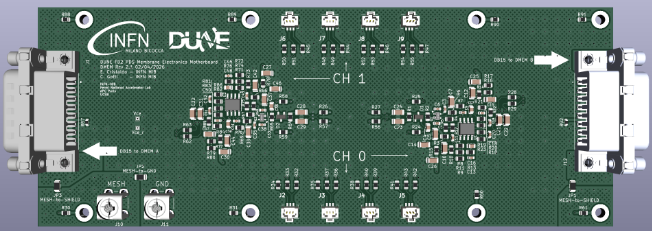
\includegraphics[width=\linewidth,height=0.205\textheight,keepaspectratio]{image7.png}
\vspace{1.1mm}
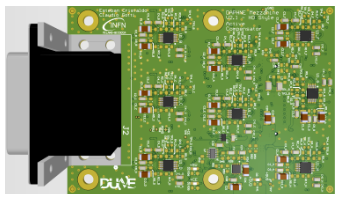
\includegraphics[width=\linewidth,height=0.255\textheight,keepaspectratio]{image5.png}

\column{0.32\linewidth}
\centering
\textbf{\small VD}\\[-0.2mm]
{\scriptsize DVDM -- HPK membrane}\\[0.8mm]
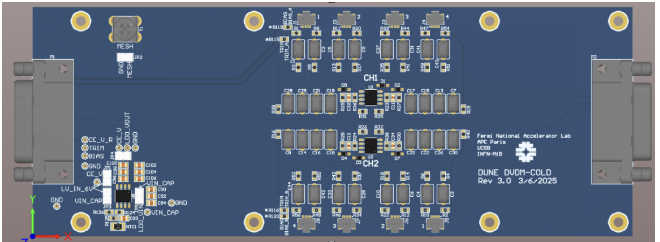
\includegraphics[width=\linewidth,height=0.205\textheight,keepaspectratio]{image8.png}
\vspace{1.1mm}
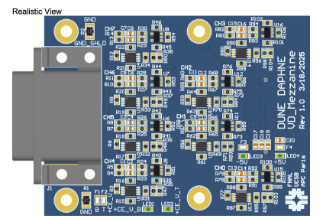
\includegraphics[width=\linewidth,height=0.255\textheight,keepaspectratio]{image4.png}

\column{0.32\linewidth}
\centering
\textbf{\small SoF}\\[-0.2mm]
{\scriptsize DCEM -- HPK cathode}\\[0.8mm]
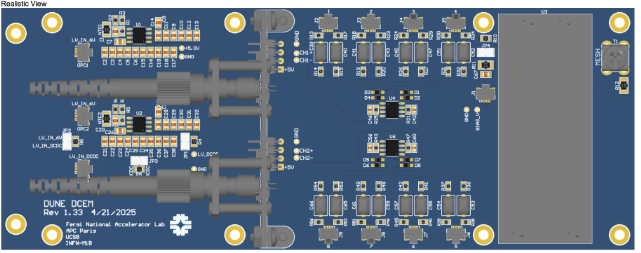
\includegraphics[width=\linewidth,height=0.205\textheight,keepaspectratio]{image9.png}
\vspace{1.1mm}
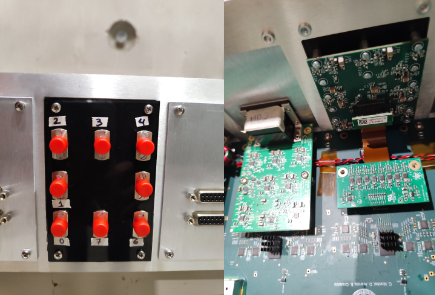
\includegraphics[width=\linewidth,height=0.255\textheight,keepaspectratio]{image6.png}
\end{columns}

\vspace{0.3mm}
\begin{beamercolorbox}[wd=\linewidth,sep=5pt,rounded=true]{panel}
\scriptsize
\textbf{Integration result:} HD, VD, and SoF cold-electronics flavors each have a matched mezzanine integration. The SoF flavor is the one that uses the two-board mechanical split with a flex-cable interface.
\end{beamercolorbox}
\end{frame}

\begin{frame}[t]{Mezzanine Evidence: Functions Under Test}
\contentdrop
\begin{columns}[T,onlytextwidth]
\column{0.32\linewidth}
\centering
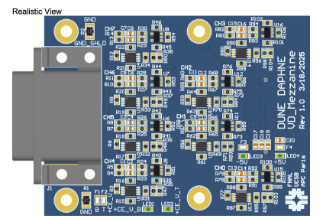
\includegraphics[width=\linewidth,height=0.32\textheight,keepaspectratio]{image4.png}
\column{0.32\linewidth}
\centering
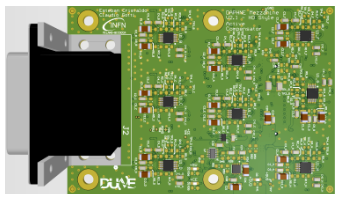
\includegraphics[width=\linewidth,height=0.32\textheight,keepaspectratio]{image5.png}
\column{0.32\linewidth}
\centering
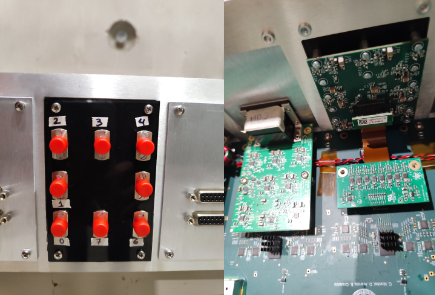
\includegraphics[width=\linewidth,height=0.32\textheight,keepaspectratio]{image6.png}
\end{columns}
\vspace{3mm}
\begin{columns}[T,onlytextwidth]
\column{0.32\linewidth}
\fixedpanelbox[panel evidence]{23mm}{Signal chain}{Active differential-to-single-ended conversion followed by AFE compensation for undershoot reduction.}
\column{0.32\linewidth}
\fixedpanelbox[panel hardware]{23mm}{Power protection}{Fused +5 V and +3.3 V cold-electronics rails, remote shutdown, power metering, and configurable overcurrent protection.}
\column{0.32\linewidth}
\fixedpanelbox[panel integration]{23mm}{Flavor coverage}{HD, VD, and SoF integrations are represented; the two-board flex-cable mechanical split applies to SoF.}
\end{columns}
\end{frame}

\begin{frame}[t]{Mezzanine Evidence: Installed Cold-Box Chain}
\softcontentdrop
\begin{columns}[T,onlytextwidth]
\column{0.48\linewidth}
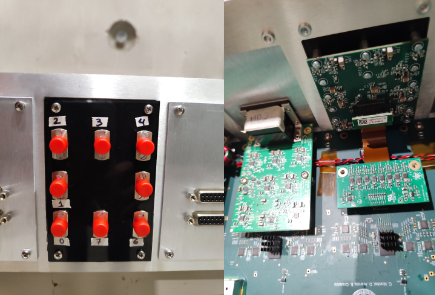
\includegraphics[width=\linewidth,height=0.50\textheight,keepaspectratio]{image6.png}

\column{0.48\linewidth}
\centering
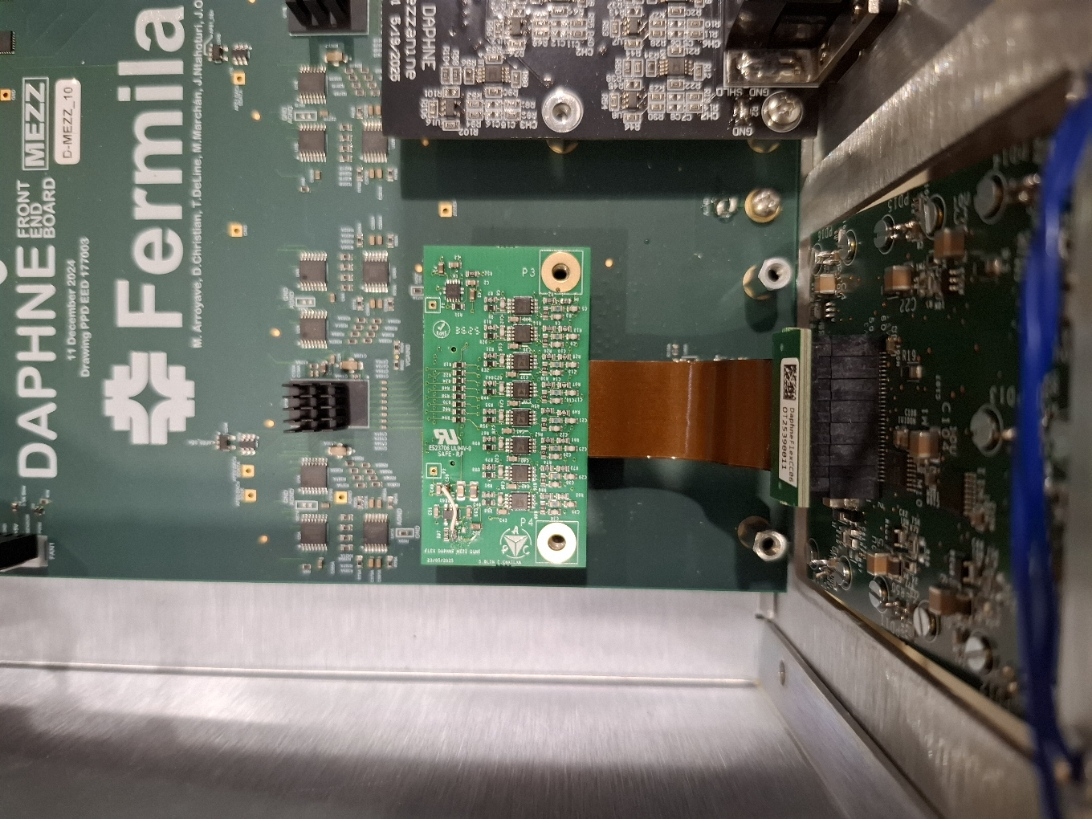
\includegraphics[height=0.42\textheight,keepaspectratio,angle=-90]{image10.jpg}
\end{columns}
\vspace{1.5mm}
\begin{beamercolorbox}[wd=\linewidth,sep=4pt,rounded=true]{panel}
\scriptsize
\textbf{Installed path:} front-panel optical input with transimpedance readout and slow-control ADC offset measurements; second board with AFE compensator, flex cable, and DAPHNE interface.
\end{beamercolorbox}
\end{frame}

\begin{frame}[t]{Mezzanine Evidence Map: Three Tests}
\begin{columns}[T,onlytextwidth]
\column{0.32\linewidth}
\fixedstatcard[panel evidence]{18mm}{1A. Signal quality}{Cold-box tests in November 2025 and January 2026 showed SNR \(>4\) for the 1500 P.E. dynamic-range setting.}
\column{0.32\linewidth}
\fixedstatcard[panel integration]{18mm}{1B. Pulse recovery}{AFE compensation reduced undershoot from around 30\% to 0.23\%.}
\column{0.32\linewidth}
\fixedstatcard[panel prr]{18mm}{1C. Dynamic range}{Membrane and cathode cold-box measurements reached the production target region near 2000 P.E.}
\end{columns}
\vspace{2mm}
\begin{beamercolorbox}[wd=\linewidth,sep=5pt,rounded=true]{panel}
\small
\textbf{SNR definition used below:} SNR versus dynamic range is calculated as \(2^{14}/A_{1\,\mathrm{P.E.}}\). The requirement statement is kept tied to the same module IDs and cold-box conditions as the plots.
\end{beamercolorbox}
\vspace{0.5mm}
\begin{beamercolorbox}[wd=\linewidth,sep=6pt,rounded=true]{panel}
\small
\textbf{Conference use:} the next slides are one evidence package, not separate topics: they show that the measured mezzanine chain preserves signal quality, waveform recovery, and usable range.
\end{beamercolorbox}
\end{frame}

\begin{frame}[t]{SNR Result: Cold-Box Curves Clear Threshold}
\figurebreath
\begin{columns}[T,onlytextwidth]
\column{0.49\linewidth}
\plotbox{0.72\textheight}{image11.png}
\column{0.49\linewidth}
\plotbox{0.72\textheight}{image12.png}
\end{columns}
\end{frame}

\begin{frame}[t]{SNR Result: All Modules Clear \(>4\)}
\centering
\figurebreath
\plotbox{0.78\textheight}{image13.png}
\end{frame}

\begin{frame}[t]{Pulse-Shape Evidence: Compensation Method}
\vspace*{6mm}
\begin{columns}[T,onlytextwidth]
\column{0.52\linewidth}
\begin{beamercolorbox}[wd=\linewidth,sep=6pt,rounded=true]{panel evidence}
\small
\textbf{Result:} the active differential-to-single-ended stage followed by the AFE compensator reduced undershoot from around 30\% to as low as 0.23\%.
\end{beamercolorbox}
\vspace{3mm}
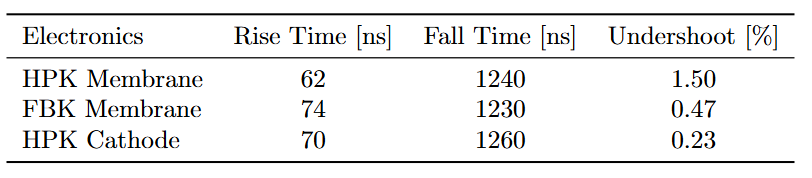
\includegraphics[width=\linewidth,height=0.25\textheight,keepaspectratio]{image17.png}

\column{0.43\linewidth}
\begin{beamercolorbox}[wd=\linewidth,sep=5pt,rounded=true]{panel}
\small
\textbf{Why it matters:} the pulse-shape correction is not only a cosmetic waveform improvement; it protects baseline recovery and keeps the downstream AFE/DAPHNE path compatible with larger light signals.
\end{beamercolorbox}
\vspace{2mm}
\begin{beamercolorbox}[wd=\linewidth,sep=5pt,rounded=true]{panel hardware}
\small
\textbf{PRR implication:} keep the compensation setting, module ID, and residual undershoot table tied to the cold-box evidence packet.
\end{beamercolorbox}
\end{columns}
\end{frame}

\begin{frame}[t]{Pulse-Shape Result: Undershoot Reduced To 0.23\%}
\figurebreath
\begin{columns}[T,onlytextwidth]
\column{0.49\linewidth}
\plotbox{0.72\textheight}{image15.png}
\column{0.49\linewidth}
\plotbox{0.72\textheight}{image16.png}
\end{columns}
\end{frame}

\begin{frame}[t]{Dynamic-Range Evidence: Measurement Method}
\begin{columns}[T,onlytextwidth]
\column{0.49\linewidth}
\fixedxlargepanelbox[panel evidence]{20mm}{Membrane run}{During the March 2026 Cold Box run, saturation was measured by increasing LED intensity with DAPHNE set to high front-end attenuation.}
\vspace{0.4mm}
\fixedxlargepanelbox[panel]{20mm}{Saturation point}{The GoF-vs-amplitude curve defines saturation from the intersection between the saturated plateau and the linear degradation region.}

\column{0.49\linewidth}
\fixedxlargepanelbox[panel prr]{20mm}{Membrane result}{FBK at +7 V and HPK at +5 V reached dynamic ranges near 2000 P.E. even at high overvoltage settings.}
\vspace{0.4mm}
\fixedxlargepanelbox[panel integration]{20mm}{Cathode reference}{The April 2024 Cold Box cathode measurement reached 2000 P.E. before saturation.}
\end{columns}
\end{frame}

\begin{frame}[t]{Dynamic-Range Result: Membrane Near 2000 P.E.}
\figurebreath
\begin{columns}[T,onlytextwidth]
\column{0.49\linewidth}
\plotbox{0.72\textheight}{image18.png}
\column{0.49\linewidth}
\plotbox{0.72\textheight}{image19.png}
\end{columns}
\end{frame}

\begin{frame}[t]{Dynamic-Range Result: Cathode Reaches 2000 P.E.}
\centering
\plotbox{0.81\textheight}{image20.png}
\end{frame}

\begin{frame}[t]{New-DAPHNE Gate: Common-Mode Noise}
\vspace*{5mm}
\begin{columns}[T,onlytextwidth]
\column{0.60\linewidth}
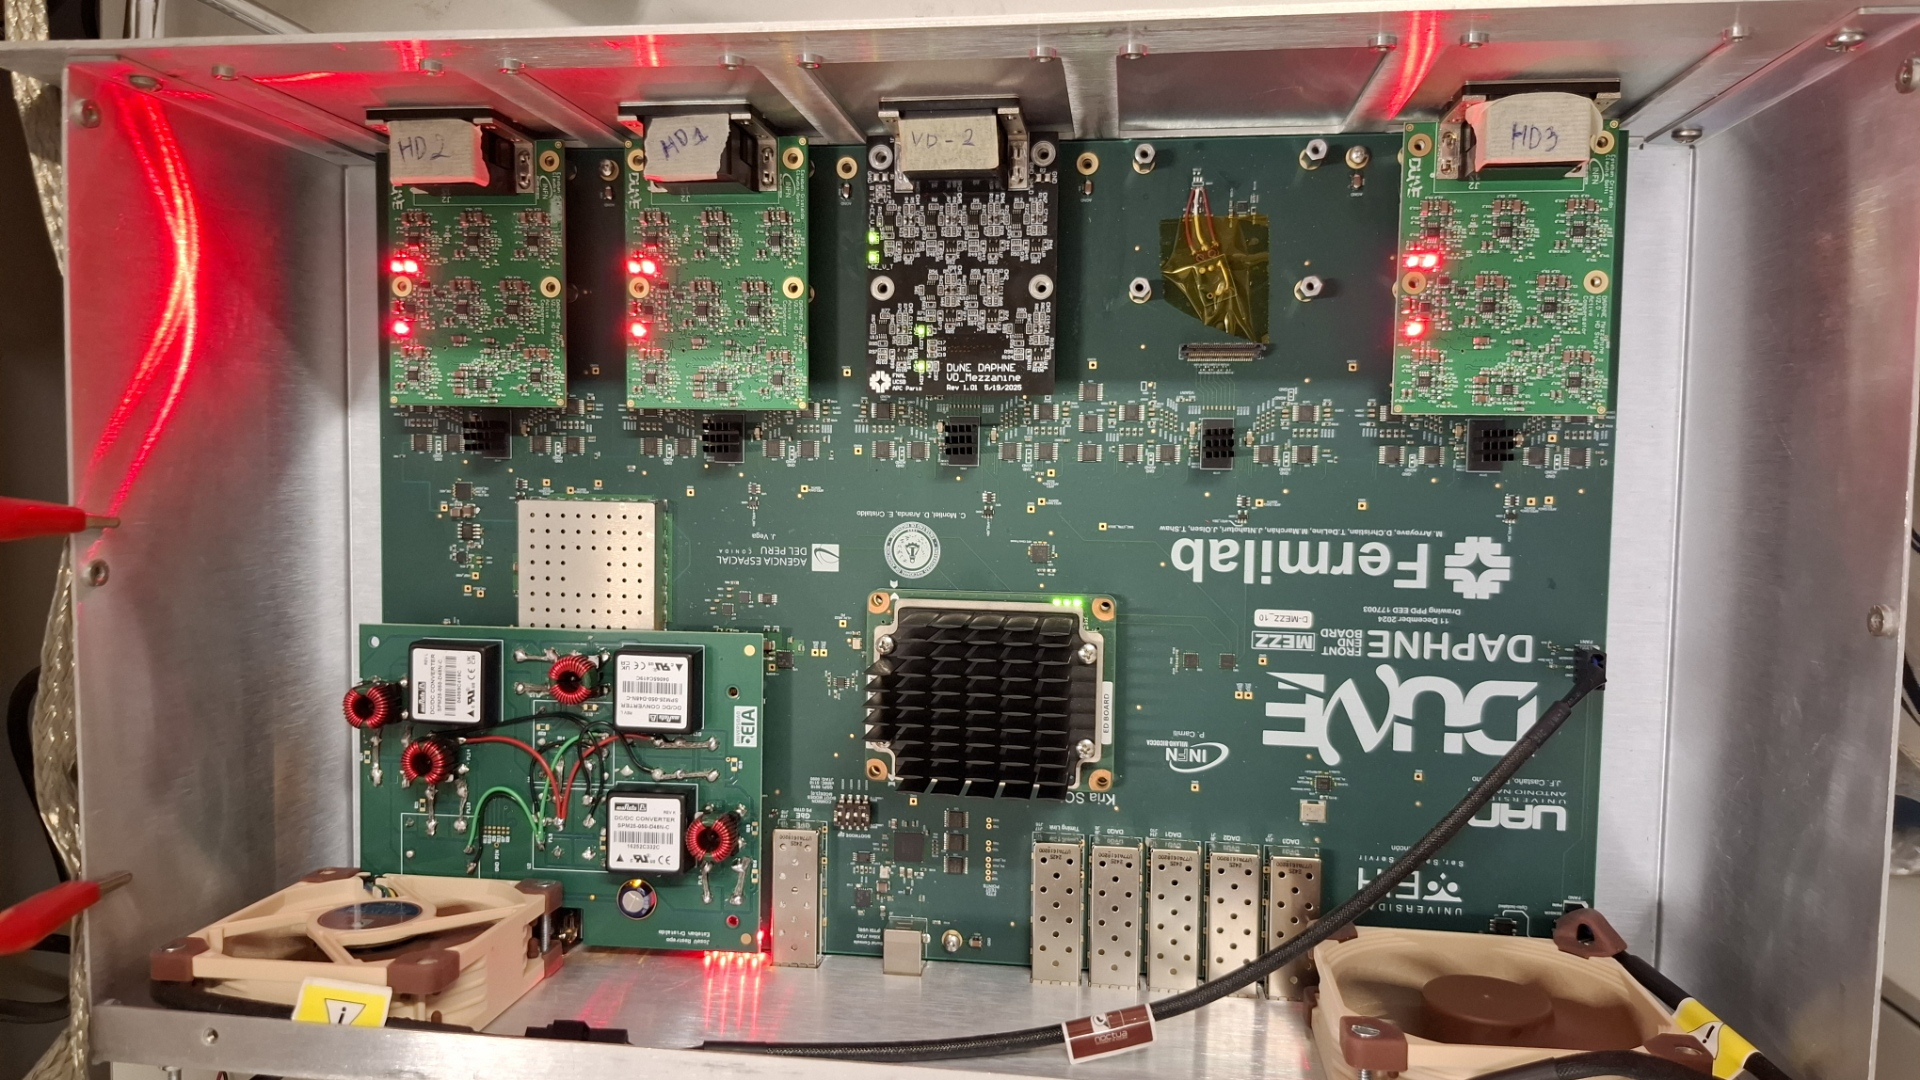
\includegraphics[width=\linewidth,height=0.68\textheight,keepaspectratio,angle=180]{image21.jpg}

\column{0.37\linewidth}
\begin{beamercolorbox}[wd=\linewidth,sep=4pt,rounded=true]{panel hardware}
\scriptsize
\textbf{Observed issue:} significant common-mode noise, especially on the SoF and HD mezzanines.
\end{beamercolorbox}
\vspace{1.4mm}
\begin{beamercolorbox}[wd=\linewidth,sep=4pt,rounded=true]{panel}
\scriptsize
\textbf{Mitigation path:} plug-in filters reduce DC/DC noise and suppress the 2 MHz spike from the -5 V charge pump.
\end{beamercolorbox}
\vspace{1.4mm}
\begin{beamercolorbox}[wd=\linewidth,sep=4pt,rounded=true]{panel prr}
\scriptsize
\textbf{Next board spin:} integrate a reduced filter plus an improved -5 V rail for lower noise.
\end{beamercolorbox}
\end{columns}
\end{frame}

\begin{frame}[t]{New-DAPHNE Gate: Filter Suppression}
\softcontentdrop
\figurebreath
\begin{columns}[T,onlytextwidth]
\column{0.49\linewidth}
\plotbox{0.70\textheight}{image22.png}
\column{0.49\linewidth}
\plotbox{0.70\textheight}{image23.png}
\end{columns}
\end{frame}

\begin{frame}[t]{DAQ/PRR Gate: Firmware Data Product}
\centering
\contentdrop
\figurebreath
\runtimeDataflowDiagram
\vspace{4mm}
\begin{beamercolorbox}[wd=\linewidth,sep=6pt,rounded=true]{panel}
\small
\textbf{DAQ contract:} firmware must make timestamp, channel identity, amplitude, timing, and descriptor validity unambiguous at the fragment boundary. Peak descriptors, x-correlation trigger logic, and dead-time mitigation remain coupled to K26 PL resource margin.
\end{beamercolorbox}
\end{frame}

\begin{frame}[t]{DAQ Integration Baseline}
\centering
\daqDiagram
\par
\begin{beamercolorbox}[wd=\linewidth,sep=4pt,rounded=true]{panel}
\small
\textbf{Status:} DAPHNE Ethernet data taking is established in DAQ. The remaining production work is to freeze the fragment schema, keep decoding in DUNE-DAQ libraries, and preserve a clean path into HDF5, monitoring, and Waffles analysis.
\end{beamercolorbox}
\end{frame}

\begin{frame}[t]{Calibration Moves Into DAQ Operations}
\centering
\softcontentdrop
\figurebreath
\pdsRunDiagram
\vspace{3mm}
\begin{beamercolorbox}[wd=\linewidth,sep=6pt,rounded=true]{panel alt}
\small
\textbf{Operational goal:} move selected calibration variables from standalone board scripts into \texttt{pds-run}, so each scan point has DAQ provenance, run control, monitoring, and reproducible configuration.
\end{beamercolorbox}
\end{frame}

\begin{frame}[t]{PRR Readiness: What Must Be Closed}
\contentdrop
\footnotesize
\setlength{\tabcolsep}{3pt}
\renewcommand{\arraystretch}{1.14}
\begin{tabularx}{\linewidth}{>{\raggedright\arraybackslash}p{0.20\linewidth} >{\raggedright\arraybackslash}X >{\raggedright\arraybackslash}p{0.25\linewidth}}
\toprule
\textbf{Area} & \textbf{Conference claim} & \textbf{PRR closure item} \\
\midrule
Mezzanine performance & \statusdot{okgreen}{SNR, pulse shape, and dynamic-range evidence in hand} & Attach test matrix, module IDs, and limitations. \\
Noise mitigation & \statusdot{warnyellow}{reduced filter path identified} & Validate on the next integrated board spin. \\
Firmware data product & \statusdot{warnyellow}{descriptor architecture is clear; resource coupling remains active} & Freeze fields, rates, and fallback modes. \\
DAQ integration & \statusdot{okgreen}{Ethernet data taking path established} & Freeze decode and schema contracts. \\
Operations and trigger & \statusdot{riskred}{scan recipes and trigger primitive ownership need closure} & Assign owners, schedule, and out-of-scope boundary. \\
\bottomrule
\end{tabularx}
\end{frame}

\begin{frame}[t]{Takeaway}
\begin{columns}[T,onlytextwidth]
\column{0.49\linewidth}
\eyebrow{WHAT WE CAN SAY}
\begin{itemize}
  \item Mezzanine analog evidence is strong and presentable.
  \item New-DAPHNE noise mitigation has a concrete closure path.
  \item DAQ integration is now part of the production story.
\end{itemize}

\column{0.49\linewidth}
\eyebrow{WHAT STILL GATES PRODUCTION}
\begin{itemize}
  \item Integrated-board noise validation.
  \item Firmware/DAQ descriptor and decode freeze.
  \item Repeatable \texttt{pds-run} operations recipes.
  \item PRR ownership for remaining trigger primitive scope.
\end{itemize}
\end{columns}
\vspace{4mm}
\begin{beamercolorbox}[wd=\linewidth,sep=6pt,rounded=true]{panel accent}
\centering

\bfseries
DAPHNE is ready to be presented as an integrated electronics-to-DAQ system, with a short and explicit production closure list.
\end{beamercolorbox}
\end{frame}

\end{document}
